\section{Results}
\label{sec:results}

% =====================================================
\subsection{Schema selection (RQ1)}
\label{sec:results-rq1}

Pooled across encoders and seeds, the 8-label entity-pair schema
(S\textsubscript{pair}) was selected for the configuration wave.
KB argmax accuracy improved by \(\Delta=+0.117\) (paired 95\% CI
[+0.045, +0.194]; Cohen's \(d=+0.55\); permutation \(p=0.015\);
FDR-\(q=0.024\)) over S\textsubscript{family} and by
\(\Delta=+0.242\) (95\% CI [+0.171, +0.313]; \(d=+1.29\);
\(p<0.0001\)) over S\textsubscript{mech} (Table~\ref{tab:t1}).
S\textsubscript{pair} outperformed S\textsubscript{family} in every
encoder (\(\Delta\in\{+0.052, +0.127, +0.132, +0.159\}\)). The
13-label schema collapsed because five of its six
drug--gene-regulation categories had no positive examples in the
BioRED test set. Per-encoder bar charts are in Figure~\ref{fig:f1};
full per-schema results are in Supplement~E.

\begin{table}[!ht]
\centering
\caption{Schema-comparison wave: pairwise contrasts on
KB argmax accuracy, paired bootstrap (\(B=10{,}000\)) on
\(4\times10=40\) matched (encoder, seed) cells.}
\label{tab:t1}
\small
\begin{tabular}{@{}lcccc@{}}
\toprule
\textbf{Contrast} & \textbf{\(\Delta\)} & \textbf{95\% CI}
& \textbf{Cohen's \(d\)} & \textbf{Perm.\ \(p\)} \\
\midrule
S\textsubscript{pair} vs S\textsubscript{family}
  & $+0.117$ & $[+0.045, +0.194]$ & $+0.55$ & $0.015$ \\
S\textsubscript{pair} vs S\textsubscript{mech}
  & $+0.242$ & $[+0.171, +0.313]$ & $+1.29$ & $<0.0001$ \\
\bottomrule
\end{tabular}
\end{table}

\begin{figure}[!ht]
\centering
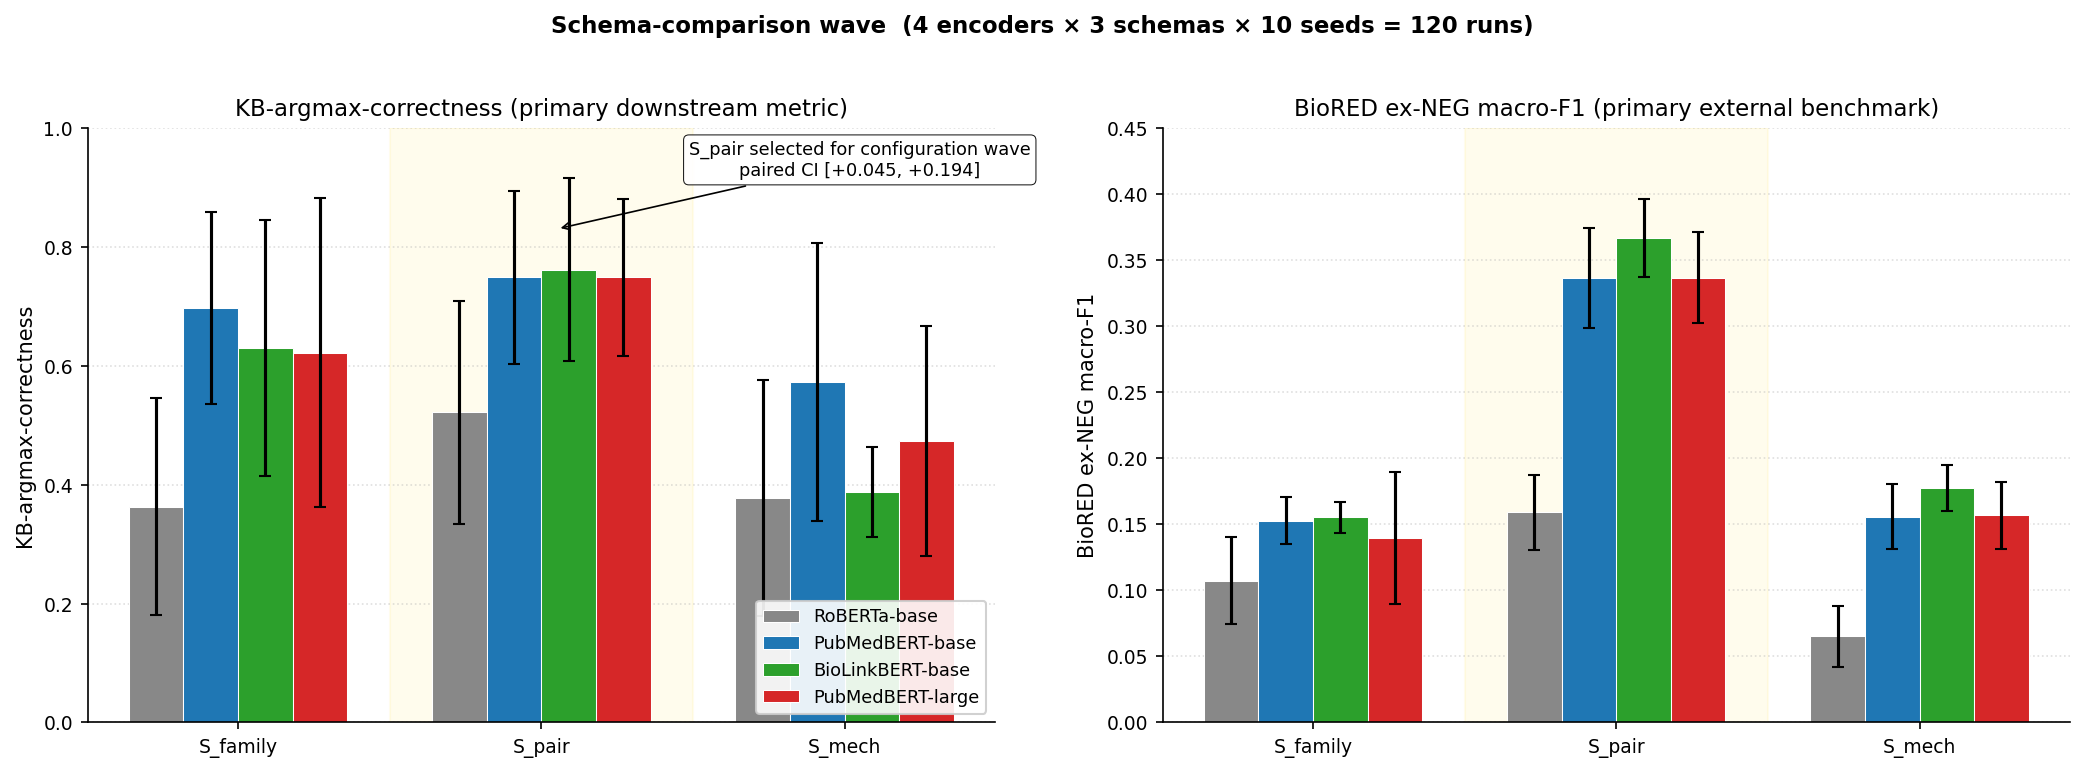
\includegraphics[width=\textwidth]{figures/fig1_schema_selection.png}
\caption{Schema-comparison wave: KB argmax accuracy (left) and
BioRED ex-NEG F1 (right) by encoder $\times$ schema. Bars are seed
means; error bars are within-cell SDs.}
\label{fig:f1}
\end{figure}

% =====================================================
\subsection{Inter-annotator audit}
\label{sec:results-iaa}

Inter-annotator agreement on a stratified 30/162 subset was
\(\kappa=0.56\) (95\% CI [0.32, 0.80]). All seven disagreements
followed a single directional pattern: the LLM annotator chose
\code{\_\_NEGATIVE\_\_} while the heuristic chose a positive
relation. The disagreements concentrated on EGFR-pathway
tyrosine-kinase inhibitors (gefitinib, erlotinib, lapatinib,
dacomitinib) and the HSP90 inhibitor tanespimycin; in six of seven
cases the CIViC-cited drug was not literally named in the abstract,
and in the seventh (gefitinib--EGFR, PMID 22370314) the gene side
was not named. The heuristic is therefore recall-favouring: it
labels too many of these abstracts as positive when one side of
the cited (drug, gene) pair is missing from the text. We retained
the heuristic unchanged and treat the audit as a directional
validity check (per-disagreement table in Supplement~C).

% =====================================================
\subsection{Training configurations (RQ2)}
\label{sec:results-rq2}

Of the nine pre-registered paired contrasts under
S\textsubscript{pair}, four confirmed, four were null, and one
marginal at \(q\approx0.05\) (Table~\ref{tab:t2}). At the family
level, the encoder-scale hypothesis (H1) was null, the
multi-corpus hypothesis (H2) was confirmed, and the staged-schedule
hypothesis (H3) was partial: 3 of 6 contrasts confirmed at
\(q<0.05\), which is the locked-design boundary between
``partial'' (2--3 of 6) and ``confirmed'' (\(\ge 4\) of 6).

\paragraph{Multi-corpus training.}
Multi-corpus joint training improved BC5CDR drug--disease F1 by
\(\Delta=+0.139\) (95\% CI [+0.108, +0.166]; Cohen's \(d=2.04\);
\(q<0.001\)) over single-corpus BioRED training at PubMedBERT-base.
The same direction held at BioLinkBERT-base (\(\Delta=+0.158\)) and
PubMedBERT-large (\(\Delta=+0.199\)).

\paragraph{Oncology-projected staging.}
Of six tests (three encoders \(\times\) two benchmarks), three
confirmed, one was marginal, and two were null. PubMedBERT-base
benefited on both benchmarks (BioRED ex-NEG \(\Delta=+0.053\),
\(q<0.001\); BC5CDR \(\Delta=+0.030\), \(q=0.007\)) and
BioLinkBERT-base on BioRED ex-NEG (\(\Delta=+0.023\), \(q=0.016\)).
PubMedBERT-large was marginal on BC5CDR drug--disease
(\(\Delta=+0.028\), \(q=0.047\)) and null on BioRED ex-NEG; staging
hurt no encoder on either benchmark. The staging benefit is real
but encoder- and benchmark-dependent.

\paragraph{Encoder scale.}
PubMedBERT-large did not outperform PubMedBERT-base
(\(\Delta=-0.008\), \(q=0.519\)) or BioLinkBERT-base
(\(\Delta=-0.021\), \(q=0.159\)) on BioRED ex-NEG. Across the
three training levers we tested, multi-corpus training produced the
largest and most reliable benchmark effect, staged continuation was
encoder-dependent, and encoder scale alone showed no benchmark
improvement at the realised cell counts. Per-cell results are in
Figure~\ref{fig:f2}; the nine paired contrasts and their CIs are in
Figure~\ref{fig:f3}; per-contrast statistics are in Supplement~F.

\begin{table}[!ht]
\centering
\caption{Configuration-wave primary-family hypothesis tests under
S\textsubscript{pair}. The Anchor column gives the
largest-magnitude paired contrast in each family. Cohen's $d$ is
$d_z$ on the paired-difference scale. Full per-contrast results
are in Supplement~F.}
\label{tab:t2}
\small
\begin{tabular}{@{}lcccp{3.5cm}@{}}
\toprule
\textbf{Test family} & \textbf{Conf.}
& \textbf{Null} & \textbf{Marg.} & \textbf{Anchor \(\Delta\) (\(d_z\))} \\
\midrule
Encoder-scale (H1; 2)    & 0 & 2 & 0 & --- \\
Multi-corpus (H2; 1)     & 1 & 0 & 0 & $+0.139$, $d_z\!=\!2.04$ (BC5CDR DD) \\
Staged schedule (H3; 6)  & 3 & 2 & 1 & $+0.053$, $d_z\!=\!0.87$ (BioRED ex-NEG) \\
\midrule
\textbf{Total (9)}       & \textbf{4} & \textbf{4} & \textbf{1} & \\
\bottomrule
\end{tabular}
\end{table}

\begin{figure}[!ht]
\centering
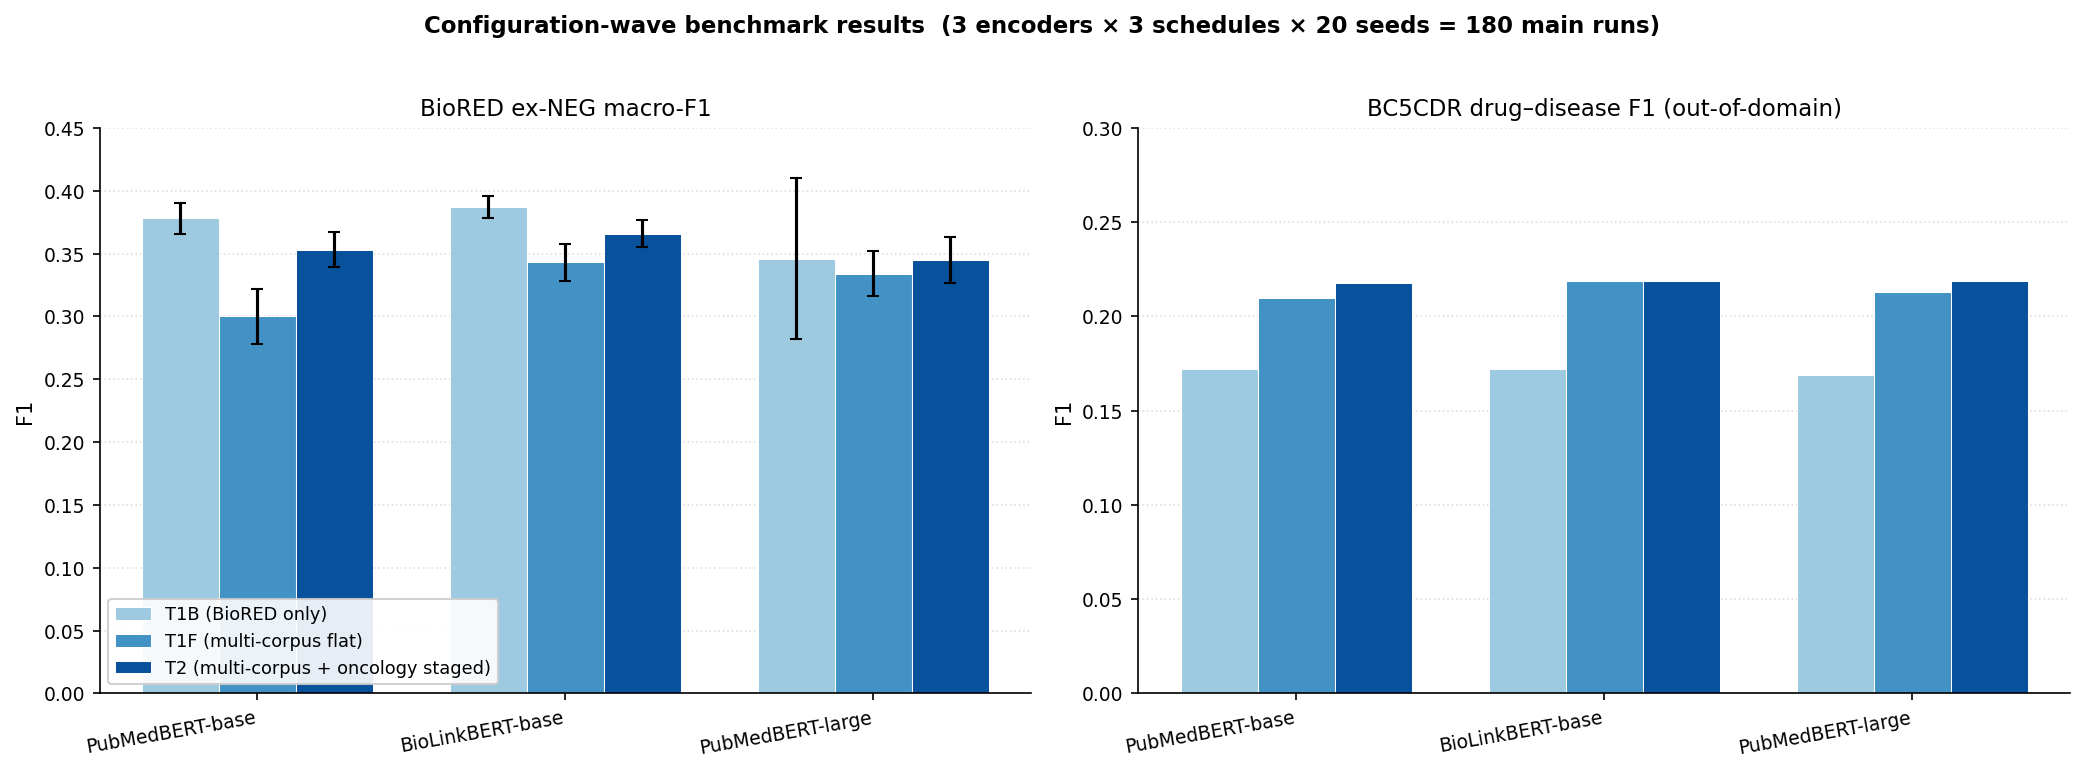
\includegraphics[width=\textwidth]{figures/fig2_training_configs_benchmarks.png}
\caption{Configuration wave: BioRED ex-NEG F1 (left) and BC5CDR
drug--disease F1 (right) by encoder $\times$ schedule. Bars are
20-seed means; error bars are within-cell SDs.}
\label{fig:f2}
\end{figure}

\begin{figure}[!ht]
\centering
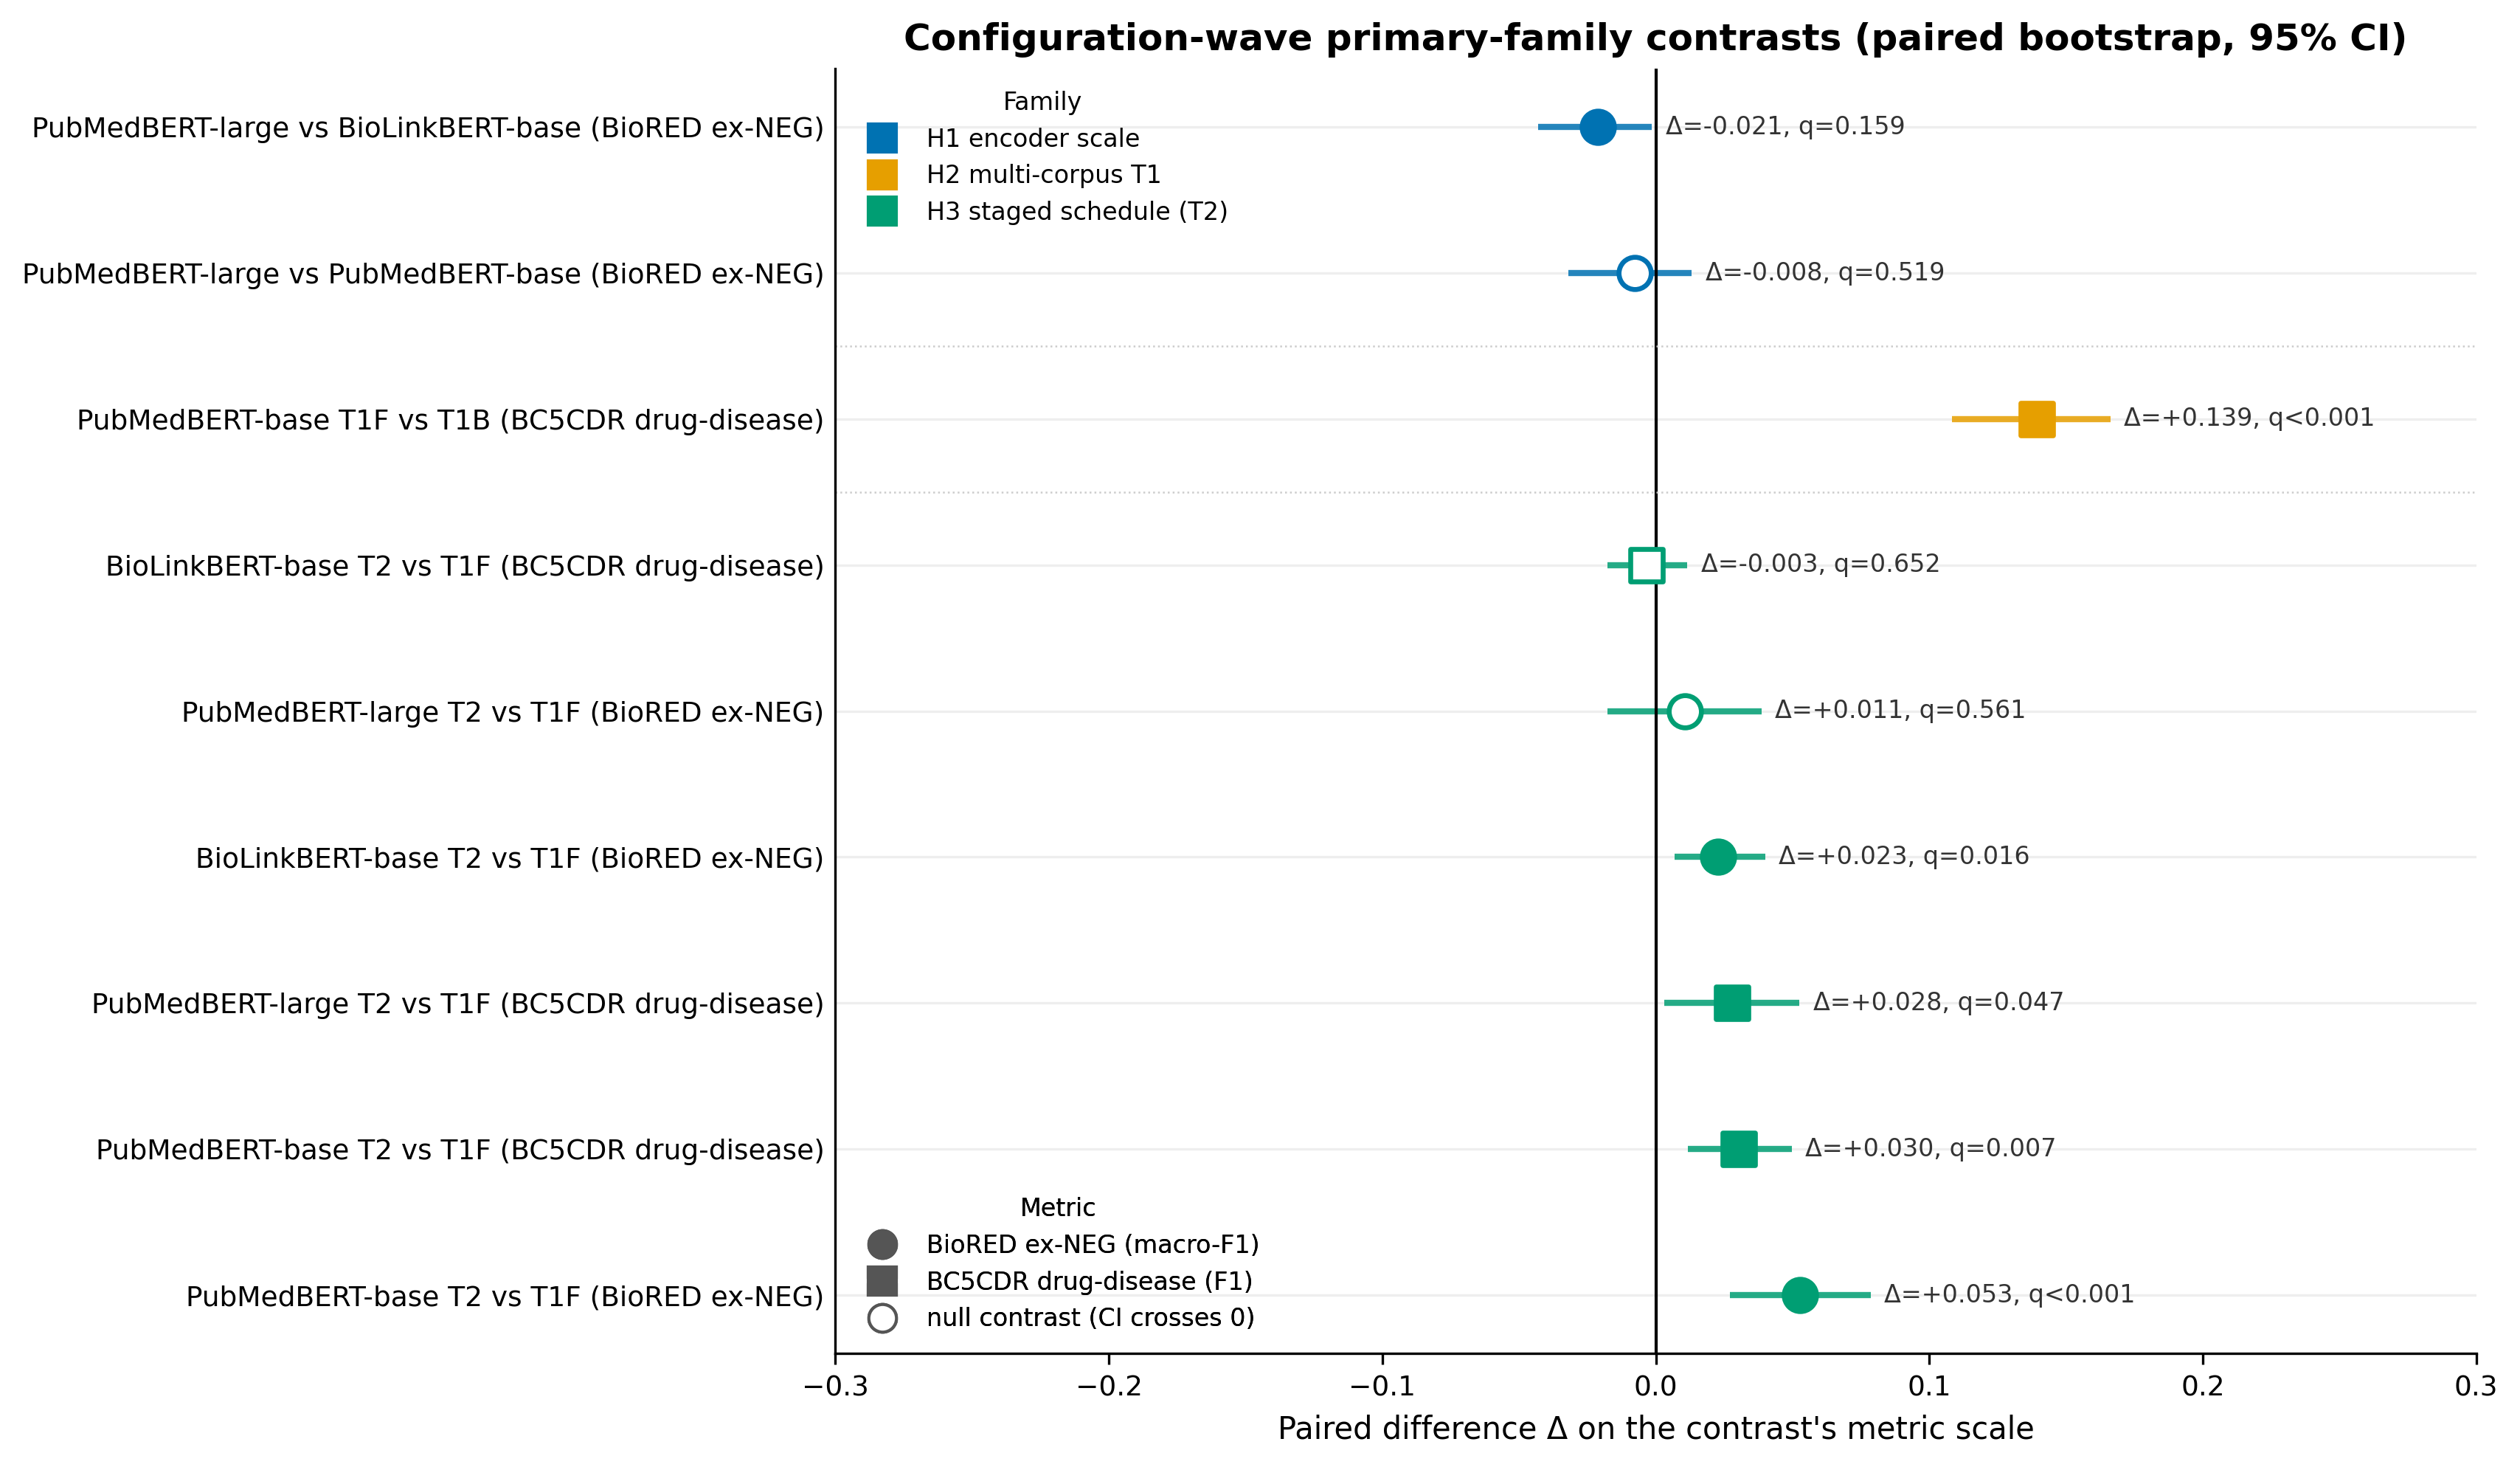
\includegraphics[width=\textwidth]{figures/fig2_forest_plot.png}
\caption{Forest plot of the nine primary-family configuration-wave
contrasts. Markers: circle = BioRED ex-NEG macro-F1; square =
BC5CDR drug--disease F1. Filled = CI excludes zero; open = null.}
\label{fig:f3}
\end{figure}

% =====================================================
\subsection{Audit-metric robustness (RQ3)}
\label{sec:results-rq3}

The encoder \(\times\) audit-metric interaction explained 0.3\% of
variance. Audit-metric choice changed absolute scale but did not
invert the encoder ordering (BioLinkBERT-base \(\approx\)
PubMedBERT-large \(>\) PubMedBERT-base across all three metrics);
the per-encoder profile across the three audit metrics is in
Figure~\ref{fig:s4-kb-profiles} (Supplement~\ref{supp:figures}).

% =====================================================
\subsection{Benchmark--KB coupling (RQ4)}
\label{sec:results-rq4}

\paragraph{Variance asymmetry.}
In the schema-comparison wave, design levers (schema, encoder, and
their interaction) explained 91.9\% of BioRED ex-NEG F1 variance
but only 40.3\% of KB argmax accuracy variance (\(R_A\approx2.28\)).
In the configuration wave the direction of the imbalance reversed:
encoder, schedule, and their interaction explained 14.2\% of
benchmark variance but 66.5\% of KB variance (\(R_B=0.21\);
cluster-bootstrap 95\% CI [0.028, 0.990]). The upper CI bound sits
immediately below unity, so we describe this as a point-estimate
direction reversal consistent with heterogeneous coupling rather
than a confirmed reversal: the test is at the boundary at the
realised cell count. The configuration-wave asymmetry is
concentrated in the schedule term, which explained 59.6\% of KB
variance but only 8.2\% of benchmark variance --- a roughly
seven-fold gap (Figure~\ref{fig:f4}; Supplement~F).

\paragraph{Rank inversion among benchmark-tied pairs.}
Of the 36 unordered configuration-cell pairs, 18 satisfied the
pre-registered matching radius \(\rho=0.03\) on BioRED ex-NEG
(approximately one schema-wave within-cell BioRED SD). Among those
18 benchmark-tied pairs, the median absolute KB argmax accuracy
difference was 0.16 and the rank-inversion rate was 0.50
(cluster-bootstrap 95\% CI [0.14, 0.83]; Clopper--Pearson exact
binomial CI [0.26, 0.74]; Figure~\ref{fig:f4}). A sensitivity
sweep over \(\rho \in \{0.01, 0.03, 0.05\}\) held the rate within
0.50--0.55 (Supplement~H). The interval does not exclude
chance-level KB ordering among benchmark-tied cells; under the
present design we read that as the substantive finding rather than
as a precision-limited null.

\paragraph{Mechanism-stratified slopes.}
All five pre-registered coupling slopes had bootstrap CI widths above
the 0.30 reportability gate and are reported as not estimable. The
configuration-arm slope was \(\beta=-3.0\) (95\% CI
[\(-13.0, +4.5\)]); the remaining four are in Supplement~G. The
reliability ceiling (\S\ref{sec:stats}) constrains slope estimation
at the realised cell counts; we draw the RQ4 coupling claim from the
variance decomposition and rank-inversion analyses above.

\begin{figure}[!ht]
\centering
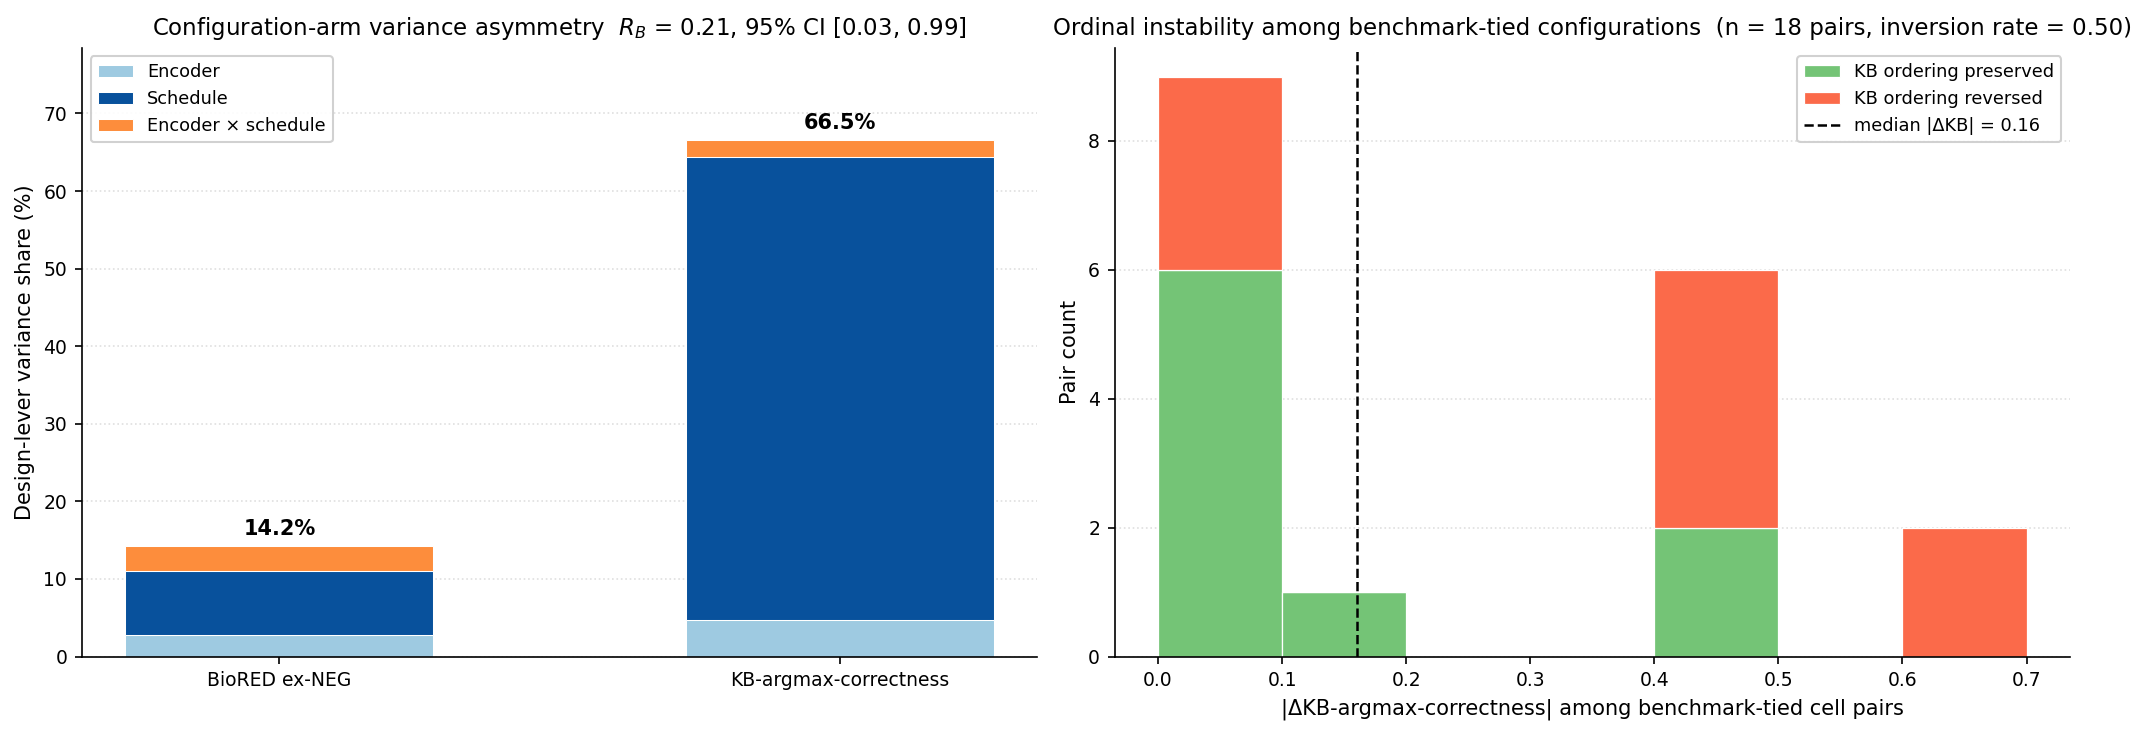
\includegraphics[width=\textwidth]{figures/fig4_variance_asymmetry_and_ordinal.png}
\caption{Left: design-lever variance shares for BioRED ex-NEG F1
and KB argmax accuracy in the configuration wave. Right:
$|\Delta\text{KB}|$ distribution among benchmark-tied cell pairs
($\rho=0.03$).}
\label{fig:f4}
\end{figure}

% =====================================================
\subsection{LoRA falsification}
\label{sec:results-lora}

All three pre-registered LoRA configurations collapsed to
predicting only the negative class (macro-F1 = 0.126, the trivial
baseline); standard fine-tuning learned meaningful predictions
within approximately 512 training steps (macro-F1 \(\approx\) 0.51).
We declared the LoRA comparison a methodological null
(Supplement~I).
